\vspace{-2mm}
\section{Architectural Template}
\label{sec:arch_template}
To implement in hardware the architectures generated by \frameworkname, we propose a PE template, shown in Figure~\ref{fig:FU_templ}. Each PE has an Instruction Memory (IM) where the operations to be performed at each clock cycle are stored. Each instruction is labeled with the clock cycle in which it should be scheduled. An internal clock counter is compared to the label to decide when to issue the instruction. The internal Register Files (RFs) are used to store input data that needs to be processed in the future, as well as output data that needs to be reused. The white rectangles in the diagram represent configurable crossbars, which can send data from any input port to any output port. OP is the hardware unit that performs an arithmetic (or logical) operation - e.g. add or multiply.
This PE template allows modular implementation of the spatial processor architecture - given that the instructions to execute are stored the local IM. The inputs to a PE can either be generated by other PEs or the output generated by the same PE in the previous clock cycle. In addition, the inputs to the PE can be used as operands for immediate computation or stored in the RFs for future use. We have implemented the template PE in RTL that can be configured to build all types of PEs found in the architectures generated by \frameworkname.

\begin{figure}[tb]
\centering
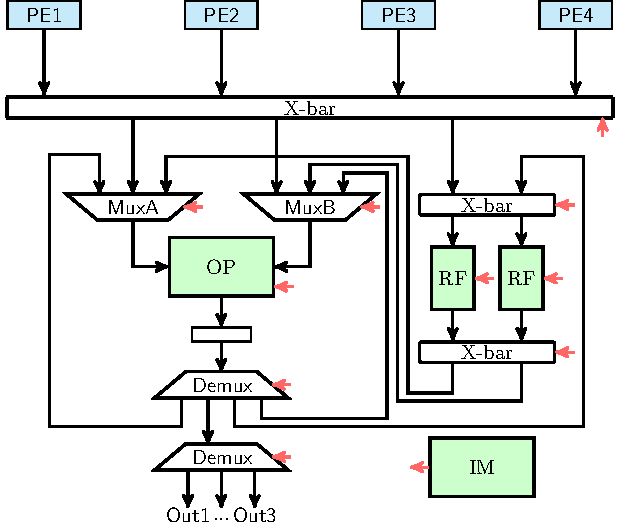
\includegraphics[width=.7\columnwidth]{images/functional_unit.pdf}
    \caption{\small Functional Unit template. PE1-PE4 represent "parent" PEs that generate input data. IM is an internal Instruction Memory,where the PE stores the operations to be performed. RFs are internal Register Files, which store reuse data and inputs to be used in the future. OP is the hardware unit actually performing the PE operation.}
\label{fig:FU_templ}
\end{figure}
